\begin{frame}\frametitle{\vspace*{0.5cm}We simulated and US-pulse impinging on a water-air interface}
  \begin{minipage}{0.62\textwidth}
    \begin{minipage}{\textwidth}
      \begin{figure}
        \centering
        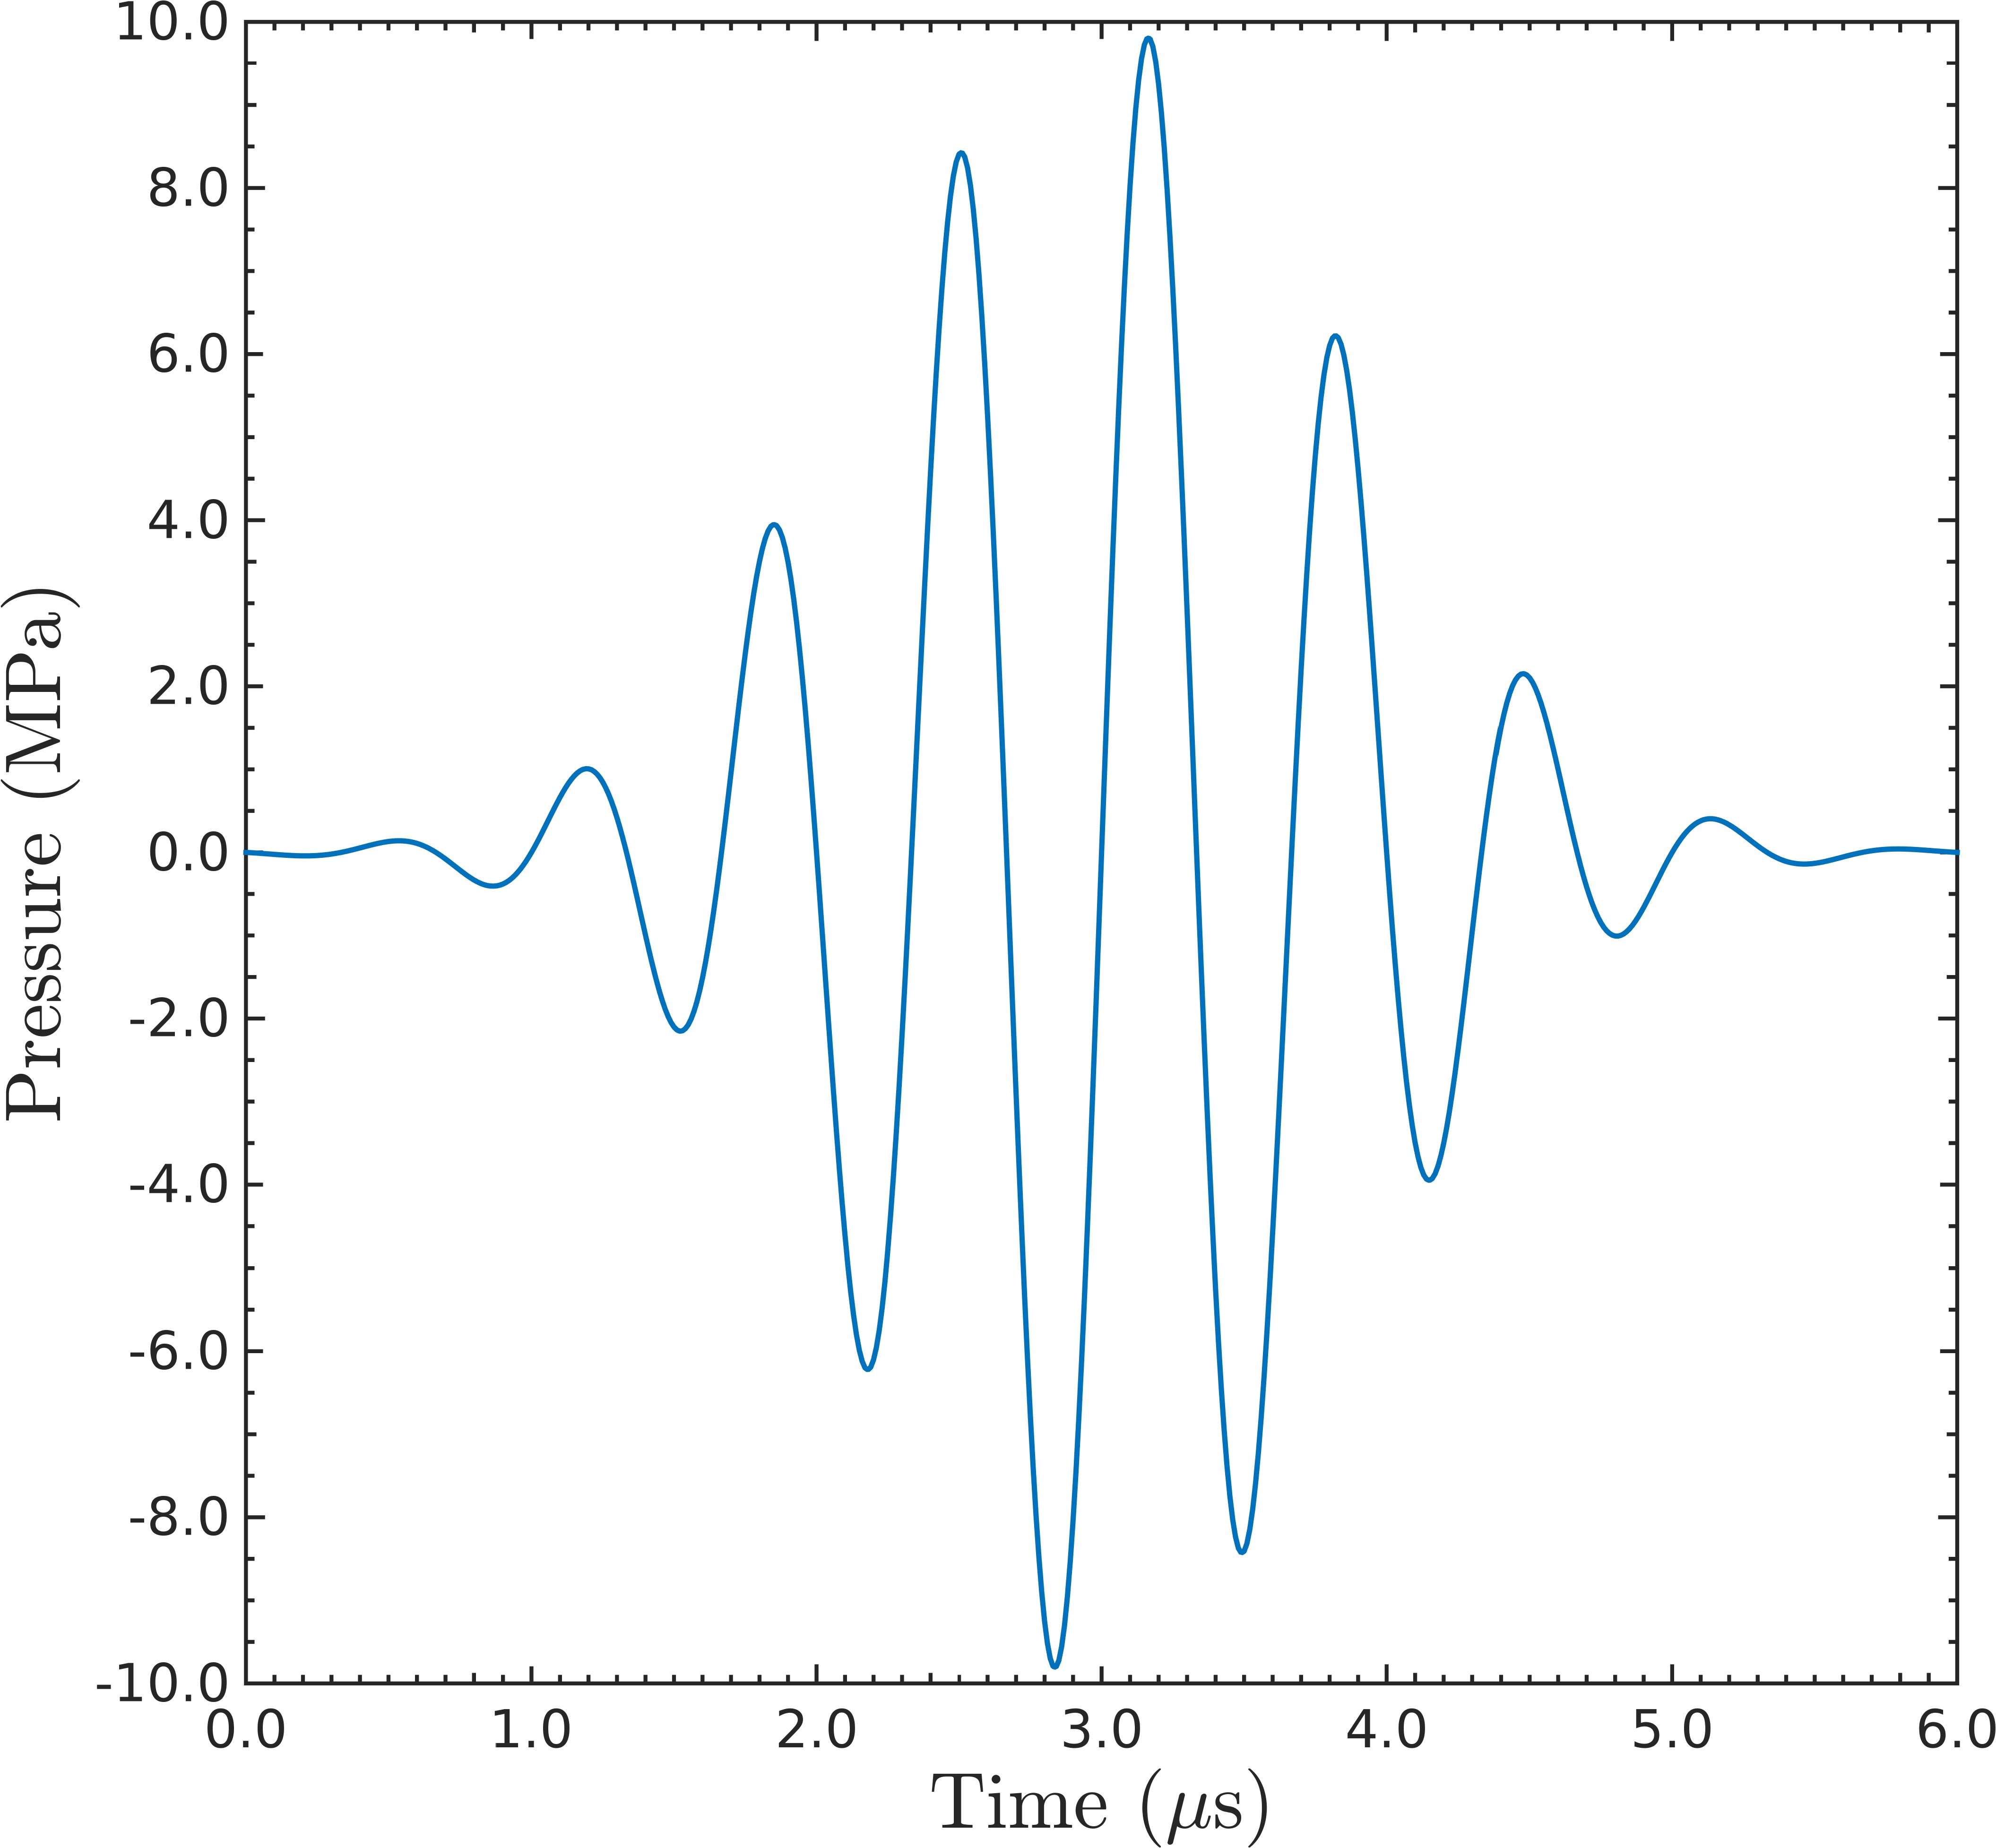
\includegraphics[width=0.47\textwidth]{../figs/lung_figs/p0_vs_t_us}%
         \def\svgwidth{0.48\textwidth} {\footnotesize
           \import{../figs/lung_figs/}{Alveolus_US_zoom_only_diagram.pdf_tex}
          \hfill%
        }%
      \end{figure}
    \end{minipage}
  % 
  \end{minipage}
  % 
  \hfill
  %
  \begin{minipage}{0.36\textwidth}
    \movie[externalviewer]{%
      \begin{tikzpicture}
          \node[anchor=south west,inner sep=0] (image) at (0,0) {
            \adjincludegraphics[trim={{0.32\width} 0 {0.32\width} 0 },clip=true,height = 0.7\textheight]{./figs/still.jpg}%x
          };%
          \begin{scope}[x={(image.south east)},y={(image.north west)}]%
            \node[font=\tiny,right] at (0.20,0.8) {Water};%
            \node[font=\tiny,right] at (0.20,0.4) {Air};%
            \node[font=\tiny,right] at (0.55,0.85) {Wave};%
            \draw[thick,->] (0.66,0.83) -- (0.66,0.75);%
          \end{scope}%  
        \end{tikzpicture}%
      }%
    {./figs/rmawave_1_10000000.0_0.03_45.0_0.0_1.0_1.0_100_100_blue.avi}
  \end{minipage}
  \vspace*{0.5cm}
  \begin{center}
      \begin{itemize}
      \item Qualitatively this looks like the interface for the trapezoidal wave.
      \item Longer simulations are needed to check late-time behavior.
      \end{itemize}
  \end{center}
  %
\end{frame}

%%% Local Variables:
%%% mode: latex
%%% TeX-master: "../main"
%%% End:
